\svnid{$Id: rt_guide.tex 1 2015-08-30 15:39:28Z rodriqu_dd $}

\chapter{Piping\label{chap:piping}}

\section{Inleiding}
Dit hoofdstuk beschrijft de procedure om een piping berekening op te zetten en uit te voeren. 

\section{Toevoegen van een piping faalmechanisme}
\label{sec:addpiping}
Om een piping berekening uit te voeren, moet er allereerst een RT project aangemaakt zijn in het algemeen project. Een RT project wordt toegevoegd in het \textbf{Project} toolvenster. Door op het project met de rechter muisknop te klikken, en dan door voor de opties \textit{New} en vervolgens \textit{Item} te kiezen.

\begin{figure} [H]
	\centering
		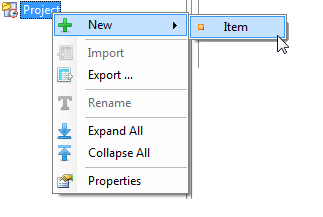
\includegraphics{figures/chapter_piping/addNewProject}
	\caption{Nieuw item toevoegen.}
	\label{fig:fig5.1}
\end{figure}

In de dialoog die dan te zien is, moet er gekozen worden voor een RT project:

\begin{figure} [H]
	\centering
		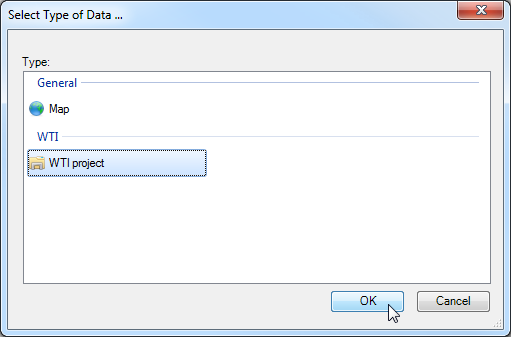
\includegraphics{figures/chapter_piping/selectRTProject}
	\caption{Nieuw toe te voegen item is RT project.}
	\label{fig:fig5.2}
\end{figure}

Door gebruik te maken van het contextmenu van het RT project, kan er uiteindelijk een piping faalmechanisme toegevoegd worden.

\begin{figure} [H]
	\centering
		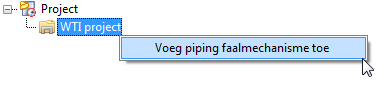
\includegraphics{figures/chapter_piping/addPipingMechanismToProject}
	\caption{Toevoeging van faalmechanisme Piping aan RT project.}
	\label{fig:fig5.3}
\end{figure}


\section{Opbouw van het faalmechanisme}

\begin{figure} [H]
	\centering
		%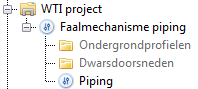
\includegraphics{figures/chapter_piping/OpbouwFaalmechanisme}
	\caption{Opbouw van het faalmechanisme}
	\label{fig:fig5.4}
\end{figure}

Het faalmechanisme kent 3 onderdelen:
\begin{enumerate}
\item \textbf{Ondergrondprofielen}. Door gebruik te maken van het contextmenu kan een .soil database met de stochastische schematisatie van de
ondergrond (SOS database) worden ge\"{i}mporteerd.
\item \textbf{Dwarsdoorsneden}. Door gebruik te maken van het contextmenu kan een .soil database met de stochastische schematisatie van de
ondergrond (SOS database) worden ge\"{i}mporteerd.
\item \textbf{Piping}. In het \textbf{Properties} venster kunnen de piping varaiabelen worden aangepast:
\begin{figure} [H]
	\centering
		%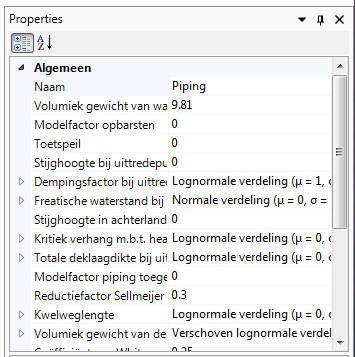
\includegraphics{figures/chapter_piping/PipingProperties}
	\caption{Aan te passen piping variabelen}
	\label{fig:fig5.5}
\end{figure}
	\begin{itemize}
	\item \textbf{Naam}: Naam van de berekening, door de gebruiker te wijzigen
	\item \textbf{Volumiek gewicht van water}: Het volumegewicht  $\gamma$ \textsubscript{water}  is ca. 10 kN/m\textsuperscript{3}
	\item \textbf{Modelfactor opbarsten}: Rekenwaarde van de modelonzekerheid
	\item \textbf{Toetspeil}: Het door HydraRing berekende toetspeil voor dit dijkvak
	\item \textbf{Stijghoogte bij uittredepunt}: 
	\item \textbf{Dempingsfactor bij uittredepunt}: Stochast; Relateert respons van stijghoogte bij binnenteen aan buitenwaterstand
	\item \textbf{Freatische waterstand bij uittredepunt}: Stochast; 
	\item \textbf{Stijghoogte in achterland}: 
	\item \textbf{Kritiek verhang m.b.t. heave}: Stochast; 
	\item \textbf{Totale deklaagdikte bij uittredepunt}: Stohast; Dikte van de laag boven de aquifer tot aan maaiveld of onderkant sloot
	\item \textbf{Modelfactor piping toegepast op Sellmeijermodel}: Rekenwaarde van de modelonzekerheid
	\item \textbf{Reductiefactor Sellmeijer}: 
	\item \textbf{Kwelweglengte}: De horizontale afstand tussen intrede- en uittredepunt die het kwelwater in de aquifer aflegt
	\item \textbf{Volumiek gewicht van de zandkorrels onder water}: Stochast; Het (ondergedompelde) volumegewicht van de korrels in de zandlaag.
	\item \textbf{Co\"{e}ffici\"{e}nt van White}: Sleepkrachtfactor volgens White
	\item \textbf{70\%-fraktiel van de korreldiameter in de bovenste zandlaag}: Stochast; Zeefmaat waar 70 gewichtsprocent van de korrels doorheen gaat. Hier de korreldiameter van het bovenste gedeelte van de aquifer, zonder de fijne fractie (<63$\mu$ meter)
	\item \textbf{Doorlatendheid aquifer}: Stochast; Darcy-snelheid waarmee water door de eerste zandlaag stroomt
	\item \textbf{Kinematische viscositeit van water bij 10\textsuperscript{$\circ$} Celsius}: 
	\item \textbf{Valversnelling}: Versnelling van de zwaartekracht [m/s\textsuperscript{2}] $\approx$ 9.81
	\item \textbf{Dikte watervoerend pakket}: Stochast; De dikte van de zandlaag die als aquifer is benoemd
	\item \textbf{Referentiewaarde voor 70\%-fraktiel in Sellmeijer regel}: Gemiddelde d70 van de in kleine schaalproeven toegepaste zandsoorten waarop de formule van Sellmeijer is gefit = 0.000208 meter
	\item \textbf{Rolweerstandshoek}: Hoek in het krachtenevenwicht die aangeeft hoeveel de korrels weerstand beiden tegen rollen; ook beddingshoek genoemd
	\begin{figure} [H]
	\centering
		%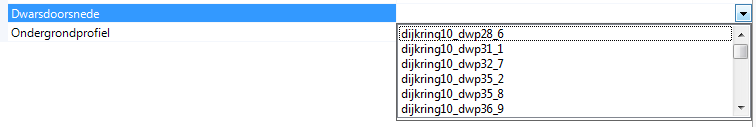
\includegraphics{figures/chapter_piping/PipingSurfacelines}
	\caption{Keuzemenu dwarsdoorsneden}
	\label{fig:fig5.6}
\end{figure}
	\item \textbf{Dwarsdoorsnede}: Keuzemenu om de dwarsdoorsnede die voor de pipingsom wordt gebruikt te selecteren die zijn opgehaald in het \textbf{Project} venster
	\item \textbf{Ondergrondprofiel}: Keuzemenu om het ondergrondprofiel die voor de pipingsom wordt gebruikt te selecteren die zijn opgehaald in het \textbf{Project} venster
	\end{itemize}

\end{enumerate}








Als alle invoergegevens voor een piping faalmechanisme berekening klaar zijn, kan deze uitgevoerd worden door op Berekenen te klikken in het contextmenu.

Als de berekening niet uitgevoerd kan worden, dan komt er een bericht terecht in het berichtpanel met verdere informatie over de reden dat het fout is gegaan. Als de berekening wel uitgevoerd is, is het resultaat toegevoegd (of ge\"{u}pdatet) in het projectpanel.





